\documentclass[11pt,a4paper]{article}
\usepackage[margin=18mm,headheight=15pt,headsep=8mm,footskip=10mm]{geometry}
\usepackage[T1]{fontenc}
\usepackage{lmodern,amsmath,amssymb,mathtools,booktabs,array,tabularx,xcolor,fancyhdr,enumitem,graphicx}
\usepackage[hidelinks]{hyperref}
\definecolor{ink}{HTML}{172B42}
\definecolor{accent}{HTML}{126A85}
\definecolor{tint}{HTML}{F0F6F8}
\definecolor{rulecolor}{HTML}{CBDDE3}
\hypersetup{pdftitle={Shor's algorithm: from entanglement to Fourier readout},pdfauthor={Prepared for Julian},pdfsubject={A merged derivation in state vectors, density matrices, and six product bases}}
\pagestyle{fancy}\fancyhf{}
\fancyhead[L]{\small\textcolor{accent}{SHOR'S ALGORITHM}}
\fancyhead[R]{\small\textcolor{ink}{States, spectra, and Fourier readout}}
\fancyfoot[L]{\small A unified explainer}
\fancyfoot[R]{\small\thepage\,/\,\pageref{docend}}
\renewcommand{\headrulewidth}{0.3pt}
\setlength{\parindent}{0pt}\setlength{\parskip}{5.5pt}
\setlength{\abovedisplayskip}{7pt}\setlength{\belowdisplayskip}{7pt}
\setlength{\abovedisplayshortskip}{4pt}\setlength{\belowdisplayshortskip}{4pt}
\setlist[itemize]{leftmargin=17pt,itemsep=2pt,topsep=3pt}
\setlist[enumerate]{leftmargin=19pt,itemsep=3pt,topsep=3pt}
\renewcommand{\arraystretch}{1.16}
\newcommand{\ket}[1]{\lvert#1\rangle}
\newcommand{\bra}[1]{\langle#1\rvert}
\newcommand{\braket}[1]{\langle#1\rangle}
\newcommand{\proj}[1]{\ket{#1}\!\bra{#1}}
\newcommand{\tr}{\operatorname{Tr}}
\newcommand{\ii}{\mathrm{i}}
\newcommand{\id}{\mathbb I}
\newcommand{\E}{\mathcal E}
\newcommand{\phead}[3]{\clearpage{\small\color{accent}\textbf{#1}}\par\vspace{2pt}{\LARGE\color{ink}\textbf{#2}}\par{\color{accent}#3}\par\vspace{6pt}}
\newcommand{\lead}[1]{\par\vspace{3pt}\textbf{\color{ink}#1}\par}
\newcommand{\takeaway}[1]{\par\smallskip\begingroup\setlength{\fboxsep}{9pt}\noindent\fcolorbox{rulecolor}{tint}{\parbox{\dimexpr\linewidth-2\fboxsep-2\fboxrule\relax}{#1}}\endgroup\par\smallskip}
\newcommand{\tight}{\fontsize{10}{12.4}\selectfont}
\newcommand{\eqsmall}{\fontsize{10}{12}\selectfont}
\begin{document}
\color{ink}\fontsize{10.5}{13.2}\selectfont
\newgeometry{left=15mm,right=15mm,top=13mm,bottom=13mm,headheight=0pt,headsep=0pt,footskip=0pt}
\thispagestyle{empty}
\begingroup
\fontsize{9.3}{11.05}\selectfont
\setlength{\parskip}{3.2pt}
\setlength{\abovedisplayskip}{4pt}\setlength{\belowdisplayskip}{4pt}
\setlength{\abovedisplayshortskip}{2pt}\setlength{\belowdisplayshortskip}{2pt}
{\fontsize{18}{20}\selectfont\bfseries\color{ink}Shor's algorithm, connected}\par
{\color{accent}Order finding is phase estimation of modular multiplication. One state connects values, combs, eigenphases, and measurable frequencies.}\par

\textbf{1. Put the period in a spectrum.}
Handle even \(N\) and prime powers classically. For remaining composite \(N\), choose \(1<a<N\). A nontrivial \(\gcd(a,N)\) already gives a factor; otherwise seek \(r=\min\{d>0:a^d\equiv1\pmod N\}\). Set \(f(x)=a^x\bmod N\), \(n=\lceil\log_2N\rceil\), and \(Q=2^t\) with \(N^2\le Q<2N^2\). Register \(C\) has \(t\) qubits, \(W\) has \(n\); \(0\le x,y<Q\), \(0\le c,s<r\). The permutation \(U_a\ket w=\ket{aw\bmod N}\), extended by identity on unused labels, cycles \(\ket{e_c}=\ket{a^c\bmod N}\) with length \(r\). For \(\omega=e^{2\pi\ii/r}\),
\[
\ket{u_s}=\frac1{\sqrt r}\sum_{c=0}^{r-1}\omega^{-sc}\ket{e_c},\qquad
U_a\ket{u_s}=\omega^s\ket{u_s},\qquad
\ket1=\frac1{\sqrt r}\sum_{s=0}^{r-1}\ket{u_s}.
\]
An index shift and roots-of-unity orthogonality prove these identities. This unknown \(r\)-point Fourier basis is analytical; the circuit uses no unknown transform.

\textbf{2. Make an eigenphase relative, efficiently.}
Control makes an unobservable global phase relative, sending
\((\alpha\ket0+\beta\ket1)\ket{u_s}\) to
\((\alpha\ket0+\beta\omega^s\ket1)\ket{u_s}\). An eigenstate target stays factored. For \(x=\sum_j2^jx_j\), the ladder
\(\Lambda=\sum_x\proj x\otimes U_a^x\) uses \(t\) controlled multipliers by \(b_j=a^{2^j}\bmod N\), computed by repeated squaring. Control phases \(2^js/r\) combine to \(\omega^{sx}\), rather than independently readable bits.

\textbf{3. Use the easy input to unite three representations.}
From \(\ket0_C\ket1_W\), \(H^{\otimes t}\) gives \(Q^{-1/2}\sum_x\ket x\ket1\); then apply \(\Lambda\). Define \(M_c=\#\{x:x\equiv c\pmod r\}=1+\lfloor(Q-1-c)/r\rfloor\) and \(\ket{C_c}=M_c^{-1/2}\sum_{m=0}^{M_c-1}\ket{c+mr}\):
\[
\begin{aligned}
\ket{\Psi_2}
&=\underbrace{\frac1{\sqrt Q}\sum_x\ket x\ket{e_{x\bmod r}}}_{\text{input/output values}}
=\underbrace{\sum_c\sqrt{M_c/Q}\ket{C_c}\ket{e_c}}_{\text{orthonormal Schmidt combs}}\\[-1pt]
&=\underbrace{\frac1{\sqrt r}\sum_s\ket{\Phi_s}\ket{u_s}}_{\text{eigenphase ramps with orthogonal work tags}},
\qquad \ket{\Phi_s}=\frac1{\sqrt Q}\sum_x e^{2\pi\ii sx/r}\ket x .
\end{aligned}
\]
Values and eigenphases describe one permutation, rather than successive gates. Easy \(\ket1\) avoids unknown eigenvector preparation. For \(r>1\), the joint state is entangled.

\textbf{4. Entanglement determines the local coherences and information.}
Ignoring \(W\) gives
\[
\rho_C=\tr_W\proj{\Psi_2}
=\sum_c\frac{M_c}{Q}\proj{C_c}=\frac1r\sum_s\proj{\Phi_s},
\qquad (\rho_C)_{xx'}=\frac1Q\mathbf1_{x\equiv x'\; (\mathrm{mod}\,r)}.
\]
The diagonal is flat: measuring now gives uniform \(x\). Identical work records preserve interference within a residue class; orthogonal records remove local cross terms between classes. The Schmidt rank is \(r\), the eigenvalues are \(\lambda_c=M_c/Q\), and
\(E=S(C)=S(W)=-\sum_c\lambda_c\log_2\lambda_c\le\log_2r\) ebits, \(S(CW)=0\), \(I(C:W)=S(C)+S(W)-S(CW)=2E\), \(S(C|W)=-E\).
If \(r\mid Q\), all \(M_c=Q/r\) and \(E=\log_2r\): \(k\) Bell pairs have \(2^k\) equal branches. When \(r\nmid Q\), the ramp ensemble is not spectral: its weights \(1/r\) are not Schmidt eigenvalues. Entropy measures information in the weights, not branch count or accessible classical bits.

\textbf{5. Phase estimation reads the frequency by interference.}
Use the known Fourier matrix \((F_Q)_{xy}=Q^{-1/2}e^{2\pi\ii xy/Q}\). Apply \(F_Q^\dagger\): each \(y\) tests frequency \(y/Q\), unwinding matching phases so amplitudes add. The QPE unitary is \((F_Q^\dagger\otimes\id)\Lambda(H^{\otimes t}\otimes\id)\), and
\[
\begin{aligned}
\ket{\Psi_3}&=\frac1{\sqrt r}\sum_{y,s}D_Q(s/r-y/Q)\ket y\ket{u_s},
&D_Q(\delta)&=\frac1Q\sum_{x=0}^{Q-1}e^{2\pi\ii x\delta},\\[-1pt]
P(y)&=\bra yF_Q^\dagger\rho_CF_Q\ket y
=\frac1r\sum_s|D_Q(s/r-y/Q)|^2,
&|D_Q(\delta)|^2&=\frac{\sin^2(\pi Q\delta)}{Q^2\sin^2(\pi\delta)}.
\end{aligned}
\]
Use continuous limits at integer \(\delta\). Orthogonal \(u_s\) tags make counting statistics an exact uniform mixture of phase-estimation laws, while \(x\)-alternatives interfere within each law. This is a statistical equivalence, not hidden branch selection. If \(r\mid Q\), outputs are \(y=sQ/r\), each with probability \(1/r\); otherwise peaks broaden. The inverse QFT need not diagonalize \(\rho_C\) and preserves \(E\). Conditioned on \(y\), the work state is \(\ket{w_y}\propto\sum_sD_Q(s/r-y/Q)\ket{u_s}\), generally a superposition.

\textbf{6. Reconstruct, verify, and factor.}
For a nearest-grid output, \(|y/Q-s/r|\le1/(2Q)<1/(2r^2)\), so the reduced fraction appears among continued-fraction convergents. Such an output has probability at least \(4/\pi^2\) per phase branch. Its denominator is \(r/\gcd(s,r)\); coprime \(s\) recovers \(r\). Repeat and verify candidates: \(a^d\equiv1\pmod N\) generally proves \(r\mid d\), not minimality alone. For even \(r\) and \(z=a^{r/2}\not\equiv\pm1\pmod N\), \(N\mid(z-1)(z+1)\) and \(\gcd(z\pm1,N)\) give factors. Retry samples or bases when necessary.

\textbf{7. Preserve the right records.}
Extra scratch multiplies \((\rho_C)_{xx'}\) by \(\langle g_{x'}|g_x\rangle\). Uncompute records distinguishing inputs inside one residue class, retaining \(f(x)\). Reversing \(\Lambda\) restores the uniform input and forces \(y=0\). Measuring \(W\)'s modular value and forgetting it removes \(C|W\) entanglement but preserves \(\rho_C\), comb coherence, and Fourier statistics. Arithmetic and reconstruction cost polynomially in \(\log N\); the QFT uses \(O(t^2)\) gates.
\par\vfill
{\fontsize{8.1}{9.3}\selectfont\color{accent}Detailed derivations: explainer Sections 3--8 and 11--15. Presentation connections and its four-branch example are integrated into the full text. All identities above allow \(r\nmid Q\), except the explicitly stated exact-peak specialization.}
\clearpage
\endgroup
\restoregeometry


{\small\color{accent}\textbf{A MERGED, SELF-CONTAINED DERIVATION}}\par
\vspace{5pt}
{\Huge\bfseries Shor's algorithm}\par
\vspace{3pt}
{\Large From entanglement to Fourier readout}\par
\vspace{8pt}
Shor finds an order by phase estimation. Modular multiplication cycles through \(r\) distinct values, so its orbit eigenphases are \(s/r\). Controlled powers write those phases into the counting register, and a known Fourier transform makes their frequencies measurable. Periodic values, Schmidt combs, and phase ramps describe the same joint state. This account connects the presentation's operator-and-phase explanation to density matrices and entanglement.

\lead{1. The problem: recover an order, then extract factors}
Given an odd composite integer \(N\), choose \(1<a<N\). If \(\gcd(a,N)>1\), a factor is already known. Otherwise define
\[
f(x)=a^x\bmod N,\qquad
r=\operatorname{ord}_N(a)=\min\{d>0:a^d\equiv1\pmod N\}.
\]
The values repeat with period \(r\), and
\[
f(x)=f(x')\quad\Longleftrightarrow\quad x\equiv x'\pmod r.
\]
Indeed, multiplying by the inverse of \(a^{x'}\) reduces equality to \(a^{x-x'}\equiv1\), which holds exactly at multiples of the order.

If \(r\) is even, set \(z=a^{r/2}\bmod N\). Then
\[
z^2\equiv1\pmod N,\qquad N\mid(z-1)(z+1).
\]
When \(z\not\equiv\pm1\pmod N\), the numbers \(\gcd(z-1,N)\) and \(\gcd(z+1,N)\) give nontrivial factors. Minimality of \(r\) rules out \(z=1\); an odd order or \(z=-1\) requires another choice of \(a\). Classical preprocessing also handles even numbers and prime powers.

\lead{The notation used throughout}
\begin{tabularx}{\linewidth}{@{}lX@{}}
\toprule
\(C,\ W\)&Counting register and work register.\\
\(Q=2^t\)&Dimension of \(C\); \(x,y\in\{0,\ldots,Q-1\}\).\\
\(r\)&Unknown order; throughout \(Q\ge r\). Standard precision uses \(N^2\le Q<2N^2\).\\
\(\ket{e_c}\)&\(\ket{a^c\bmod N}\), \(c=0,\ldots,r-1\): distinct orthogonal work states.\\
\(M_c,\ \ket{C_c}\)&Size of residue class \(c\), and its normalized periodic comb.\\
\(\omega\)&\(e^{2\pi\ii/r}\); logarithms are base \(2\).\\
\bottomrule
\end{tabularx}
\lead{A route through the document}
The opening page gives the connected derivation. Sections 2--8 explain the mechanism; new Sections 5a--5b connect Schmidt form, density matrices, and changes of basis. Sections 9--11 work through samples and factors. Sections 12--13 cover measurement and density evolution; new Section 12a explains mixed-state separability. Sections 14--17 give the basis catalog, Bell context, and sources. No classical polynomial-time algorithm is known for general order finding.

\takeaway{\textbf{What the quantum step supplies:} samples with \(y/Q\) close to \(s/r\). It does not directly print \(r\), and measuring the original input label \(x\) supplies no period information.}

\phead{FOUNDATIONS}{2. States, coherences, and local descriptions}{The small toolkit needed for every later calculation.}
A pure state is a normalized ket. A density operator satisfies \(\rho\ge0\) and \(\tr\rho=1\). Pure states have \(\rho=\proj{\psi}\), of rank one; mixtures have \(\rho=\sum_jp_j\proj{\psi_j}\). Such decompositions are nonunique. A reduced mixed state need not mean ignorance about an actual local pure state.

For two systems, \(\mathcal H_{CW}=\mathcal H_C\otimes\mathcal H_W\). If
\(\ket{\Psi}=\sum_{x,k}A_{xk}\ket{x}\ket{k}\), then
\[
(\rho_{CW})_{(x,k),(x',k')}=A_{xk}A_{x'k'}^*,
\quad
(\rho_C)_{xx'}=\sum_kA_{xk}A_{x'k}^*.
\]
The second equation is the partial trace: \(\rho_C=\tr_W\rho_{CW}\). In particular,
\[
\tr_W\!\left(A\otimes\ket v\bra w\right)=A\braket{w|v},
\qquad\braket{w|v}\equiv\langle w|v\rangle .
\]
\lead{Why off-diagonal entries matter}
In a chosen orthonormal basis, diagonal entries are measurement probabilities; off-diagonal entries encode coherence between alternatives:
\[
\proj{+}=\frac12\begin{pmatrix}1&1\\1&1\end{pmatrix},
\qquad
\frac{\id_2}{2}=\frac12\begin{pmatrix}1&0\\0&1\end{pmatrix},
\quad
\ket+=\frac{\ket0+\ket1}{\sqrt2}.
\]
Both give a fair \(0/1\) outcome. An \(X\)-basis measurement gives \(+\) certainly for the first, but a fair \(+/-\) outcome for the second. Coherence depends on the basis; the spectrum and purity do not. The presentation's smallest phase-readout experiment is
\[
H\!\begin{pmatrix}1&0\\0&e^{2\pi\ii\phi}\end{pmatrix}\!H\ket0
=\frac{1+e^{2\pi\ii\phi}}2\ket0+\frac{1-e^{2\pi\ii\phi}}2\ket1,
\quad P(0)=\cos^2(\pi\phi).
\]
Recombining the alternatives makes relative phase observable. The inverse QFT generalizes this two-path interference to \(Q\) counting alternatives.

\lead{One physical gate, acting on both sides of a density matrix}
If \(\ket{\psi'}=V\ket\psi\), then \(\bra{\psi'}=\bra\psi V^\dagger\). Hence
\[
\rho'=V\rho V^\dagger,\qquad
P(j)=\bra j\rho'\ket j.
\]
For \(V=F_Q^\dagger\), this is \(F_Q^\dagger\rho F_Q\). The right-hand \(F_Q\) comes from the bra; it is not a second physical gate.

\lead{Entanglement is a property of a specified split}
A joint state is separable if
\[
\rho_{CW}=\sum_jp_j\,\sigma_C^{(j)}\otimes\tau_W^{(j)};
\]
otherwise it is entangled. For a \emph{pure} joint state, entangled means the ket cannot factor as \(\ket c\otimes\ket w\). Equivalently its coefficient matrix \(A\) has rank greater than one, and each marginal is mixed.

A Bell pair \((\ket{00}+\ket{11})/\sqrt2\) and a shared-coin mixture
\(\frac12(\proj{00}+\proj{11})\) have the same marginals \(\id_2/2\). The former is pure and entangled; the latter is mixed and separable. Local mixedness alone therefore diagnoses entanglement only when joint purity is known.

\takeaway{Shor uses trusted quantum gates and interference, rather than a Bell test. A CHSH violation \(|\mathcal B|>2\) certifies entanglement under its experimental assumptions; entanglement itself does not imply that every state or choice of measurements violates CHSH.}

\phead{THE PHYSICAL CIRCUIT}{3. Every gate and every state}{Here arrows mean actual quantum operations; later equalities change descriptions.}
Define modular multiplication on valid work labels by \(U_a\ket z=\ket{az\bmod N}\). Since \(a\) is invertible modulo \(N\), this is a permutation; extend it unitarily on unused binary labels. In the occupied orbit, \(U_a\ket{e_c}=\ket{e_{c+1\bmod r}}\) and \(\ket{e_0}=\ket1\).

The complete ideal evolution, with scratch qubits returned to their initial state, is
\begin{align*}
\ket{\Psi_0}&=\ket0_C\ket1_W,\\
&\xrightarrow{\ H^{\otimes t}\otimes\id\ }\quad
\ket{\Psi_1}=\frac1{\sqrt Q}\sum_x\ket x\ket1,\\
&\xrightarrow{\ U_{\rm ME}\ }\quad
\ket{\Psi_2}=\frac1{\sqrt Q}\sum_x\ket x\ket{e_{x\bmod r}},\\
&\xrightarrow{\ F_Q^\dagger\otimes\id\ }\quad
\ket{\Psi_3}=\frac1Q\sum_{y,x}e^{-2\pi\ii xy/Q}
                  \ket y\ket{e_{x\bmod r}}.
\end{align*}
The final step is a computational measurement of \(C\). The Fourier sign convention is
\[
F_Q\ket y=\frac1{\sqrt Q}\sum_xe^{2\pi\ii xy/Q}\ket x.
\]
The controlled modular exponentiation is
\[
U_{\rm ME}=\sum_x\proj x\otimes U_a^x.
\]
Applying it to \(\ket x\ket1\) gives \(U_a^x\ket1=\ket{a^x\bmod N}\), proving the third line above.

\lead{Why the controlled-power ladder is efficient}
Writing the binary input as \(x=\sum_{j=0}^{t-1}2^jx_j\) gives
\[
U_a^x=\prod_{j=0}^{t-1}(U_a^{2^j})^{x_j},
\quad
U_{\rm ME}=
\prod_{j=0}^{t-1}
\left(\proj0_j\otimes\id+\proj1_j\otimes U_a^{2^j}\right).
\]
Repeated squaring computes the classical constants \(b_j=a^{2^j}\bmod N\). Each controlled power multiplies by \(b_j\), using reversible modular arithmetic. We do not perform \(x\) sequential multiplications.

After the first \(\ell\) controls, define \(p_\ell(x)=\sum_{j<\ell}2^jx_j\). The intermediate state is exactly
\[
\ket{\Psi_{2,\ell}}=\frac1{\sqrt Q}\sum_x
\ket x\ket{e_{p_\ell(x)\bmod r}}.
\]
Thus \(p_0=0\) gives \(\Psi_1\), while \(p_t=x\) gives \(\Psi_2\). This also specifies the state after every controlled multiplier.

\takeaway{The circuit prepares a superposition of correlated inputs and outputs. Its usefulness comes from how these alternatives later interfere, not from reading all the function values out of one run.}

\phead{THE WORK EIGENBASIS}{4. Where phase kickback comes from}{The periodic-tag description and the phase description are the same joint state.}
The work orbit has length \(r\), and \(U_a\) shifts its labels by one. The simplest analogue is \(X=HZH\): one map swaps computational labels and applies phases to its eigenvectors. Fourier-transform the \(r\)-state modular orbit:
\[
\ket{u_s}=\frac1{\sqrt r}\sum_{c=0}^{r-1}\omega^{-sc}\ket{e_c},
\qquad s=0,\ldots,r-1.
\]
Shifting \(d=c+1\bmod r\) proves
\[
U_a\ket{u_s}
=\frac1{\sqrt r}\sum_d\omega^{-s(d-1)}\ket{e_d}
=\omega^s\ket{u_s}.
\]
The identity \(\frac1r\sum_s\omega^{s(c-d)}=\delta_{cd}\) proves orthonormality and the inverse expansion
\[
\ket{e_c}=\frac1{\sqrt r}\sum_s\omega^{sc}\ket{u_s},
\qquad
\ket1=\ket{e_0}=\frac1{\sqrt r}\sum_s\ket{u_s}.
\]
\lead{A global phase becomes a relative phase under control}
For an eigenvector \(U\ket u=e^{\ii\theta}\ket u\),
\[
\frac{\ket0+\ket1}{\sqrt2}\ket u
\xrightarrow{\ {\rm controlled}\text{-}U\ }
\frac{\ket0+e^{\ii\theta}\ket1}{\sqrt2}\ket u.
\]
The phase multiplies only the control-\(1\) branch, so it is relative and measurable. The work eigenstate itself factors out. Linearity lets us apply this rule to every eigenstate component of the actual work input.

For the full ladder,
\[
U_a^x\ket{u_s}=\omega^{sx}\ket{u_s},
\qquad
\ket{\Phi_s}=\frac1{\sqrt Q}\sum_x\omega^{sx}\ket x.
\]
Substituting the inverse work expansion into \(\Psi_2\) gives
\[
\boxed{\;
\ket{\Psi_2}
=\frac1{\sqrt{Qr}}\sum_{x,s}\omega^{sx}\ket x\ket{u_s}
=\frac1{\sqrt r}\sum_s\ket{\Phi_s}\ket{u_s}.
\;}
\]
For one eigenphase, the counting ramp factorizes into the control-qubit phases:
\[
\ket{\Phi_s}
=\bigotimes_{j=t-1}^{0}
\frac{\ket0+e^{2\pi\ii\,2^js/r}\ket1}{\sqrt2}.
\]
Expanding this product multiplies phases: \(\prod_j\omega^{s2^jx_j}=\omega^{s\sum_j2^jx_j}=\omega^{sx}\). Bilinearity lets a scalar be collected from either tensor factor; the controlled gate places it on only one branch, making it relative. For a partial ladder, replace \(x\) by \(p_\ell(x)\).

\lead{What this expansion does, and does not, imply}
Starting \(W\) in one \(\ket{u_s}\) gives a product \(\ket{\Phi_s}\ket{u_s}\). With the actual input \(\ket1\), distinct orthogonal work eigenstates become paired with nonproportional counting ramps, so \(\Psi_2\) is entangled for \(r>1\). Equivalently, the coherent input pairs different \(x\) with distinct \(f(x)\) values; a product would require the same work vector for every \(x\). These are two descriptions of the same entanglement. The permutation's complex phases appear in its eigenbasis without an extra physical gate.

The work vectors \(\ket{u_s}\) are orthonormal, but the counting ramps \(\ket{\Phi_s}\) need not be. The displayed equal-weight expansion is therefore not automatically a Schmidt decomposition. No physical measurement has selected a hidden \(s\); it is an alternative expression for the pure joint state.

\phead{THE SCHMIDT VIEW}{5. Partial trace, periodic combs, and class sizes}{A pure global state becomes a mixed local description when its partner is ignored.}
Form the joint outer product and trace out the work tags:
\begin{align*}
\rho_2&=\frac1Q\sum_{x,x'}\ket x\bra{x'}
 \otimes\ket{e_{x\bmod r}}\bra{e_{x'\bmod r}},\\
\rho_C&=\frac1Q\sum_{x,x'}\langle e_{x'\bmod r}|e_{x\bmod r}\rangle
                  \ket x\bra{x'}\\
&=\boxed{\frac1Q\sum_{x\equiv x'\;(\mathrm{mod}\,r)}\ket x\bra{x'}}.
\end{align*}
Every diagonal entry is \(1/Q\). Off-diagonal entries survive precisely between alternatives leaving the \emph{same} work tag. Orthogonal tags erase these cross terms from the local description; they do not make the joint state mixed.

\lead{Count and normalize each residue class}
For \(Q\ge r\), define
\[
M_c=\#\{0\le x<Q:x\equiv c\pmod r\}
=\left\lfloor\frac{Q-1-c}{r}\right\rfloor+1,
\qquad \sum_cM_c=Q,
\]
\[
\ket{C_c}=\frac1{\sqrt{M_c}}\sum_{m=0}^{M_c-1}\ket{c+mr}.
\]
If \(Q=qr+\ell\), \(0\le\ell<r\), the first \(\ell\) classes have \(q+1\) labels and the rest have \(q\). The combs are orthonormal because their supports are disjoint. Grouping the sum for \(\Psi_2\) by residues proves its exact Schmidt form:
\[
\boxed{\ket{\Psi_2}=\sum_c\sqrt{\frac{M_c}{Q}}\ket{C_c}\ket{e_c}.}
\]
Consequently,
\[
\boxed{\rho_C=\sum_c\frac{M_c}{Q}\proj{C_c},
\qquad \rho_W=\sum_c\frac{M_c}{Q}\proj{e_c}.}
\]
The Schmidt coefficients are \(\sqrt{M_c/Q}\); the marginal eigenvalues are their squares, \(M_c/Q\). There are \(r\) nonzero values. The remaining \(Q-r\) counting eigenvalues are zero.

\lead{Connect this to the phase ramps}
Tracing the work eigenbasis expansion gives another exact expression:
\[
\rho_C=\frac1r\sum_s\proj{\Phi_s},
\qquad
(\rho_C)_{xx'}=\frac1{Qr}\sum_s\omega^{s(x-x')}
=\frac1Q\mathbf1_{x\equiv x'\;(\mathrm{mod}\,r)}.
\]
These are the same operator. The comb expression is spectral; the ramp expression is an ensemble, spectral only when its ramps are orthogonal. Its equal ensemble weights must not be mistaken for eigenvalues.

\phead{SCHMIDT AND DENSITY MATRICES}{5a. Why orthogonality matters}{Schmidt form reveals the spectra of both reduced states.}
A Schmidt decomposition is a coherent sum of paired, orthonormal local vectors:
\[
\ket\Psi=\sum_k\sqrt{\lambda_k}\ket{a_k}\ket{b_k},
\qquad \lambda_k>0,\quad\sum_k\lambda_k=1.
\]
Its joint density matrix contains coherence between different branch labels:
\[
\rho_{AB}=\sum_{j,k}\sqrt{\lambda_j\lambda_k}\,
\ket{a_j}\bra{a_k}\otimes\ket{b_j}\bra{b_k}.
\]
The whole state is pure: the joint spectrum is \((1,0,\ldots)\). Taking a partial trace describes access to one subsystem; it does not measure the partner or destroy the joint cross terms.

\lead{Orthogonality has a separate role on each side}
For any paired expansion of this form, before assuming orthogonality,
\[
\rho_A=\sum_{j,k}\sqrt{\lambda_j\lambda_k}\,
\braket{b_k|b_j}\ket{a_j}\bra{a_k}.
\]
Orthogonality of the traced-out vectors removes cross terms. Orthogonality of the retained vectors then makes the remaining expression spectral:
\[
\boxed{\rho_A=\sum_k\lambda_k\proj{a_k},\qquad
\rho_B=\sum_k\lambda_k\proj{b_k}.}
\]
Thus \(\rho_A\ket{a_k}=\lambda_k\ket{a_k}\), and similarly for \(B\). The nonzero reduced spectra agree, even when the subsystem dimensions differ. Schmidt amplitudes are \(\sqrt{\lambda_k}\); their squares are the marginal eigenvalues. Both local Schmidt measurements reveal the same perfectly distinguishable label \(k\), with probability \(\lambda_k\).

\lead{Counting arbitrary terms would give false entanglement}
The product state
\[
\ket0\ket+=\frac{\ket0\ket0+\ket0\ket1}{\sqrt2}
\]
has two equal terms but only one Schmidt term, \(\ket0\ket+\). Its two displayed \(A\)-vectors coincide. Treating \(1/2,1/2\) as reduced eigenvalues would incorrectly assign one ebit to a product state. A valid expansion therefore need not be Schmidt.

\lead{Construct Schmidt form by diagonalizing a marginal}
Diagonalize \(\rho_A\), keeping its positive eigenvalues and corresponding orthonormal eigenvectors. Define
\[
\ket{b_k}=\frac{(\bra{a_k}\otimes\id_B)\ket\Psi}{\sqrt{\lambda_k}},
\qquad
\braket{b_j|b_k}
=\frac{\bra{a_k}\rho_A\ket{a_j}}{\sqrt{\lambda_j\lambda_k}}
=\delta_{jk}.
\]
These partner vectors reconstruct \(\Psi\) and are automatically orthonormal. Every pure bipartite state therefore admits Schmidt form. Equivalently, it is the singular-value decomposition of the ket's coefficient matrix; squared singular values give the reduced eigenvalues.

\takeaway{For Shor, \(\lambda_c=M_c/Q\), \(\ket{a_c}=\ket{C_c}\), and \(\ket{b_c}=\ket{e_c}\). Rank \(r>1\) proves entanglement because the coherent input pairs orthogonal combs with distinct modular values. The input/output and eigenphase expressions describe this same state in different work bases.}

\phead{SCHMIDT BASES AND PHASE RAMPS}{5b. Which basis changes preserve Schmidt form?}{A fixed spectrum allows rotations only within equal-weight blocks.}
For distinct positive \(\lambda_k\), the paired Schmidt vectors are fixed up to reordering and compensating phases. Equal eigenvalues permit compensated unitary rotations within their common eigenspaces. Arbitrary changes of product basis still describe the state, but generally lose Schmidt form.

\lead{Equal comb weights give many Schmidt decompositions}
If \(r\mid Q\), all occupied eigenvalues are \(1/r\). For any unitary \(r\times r\) matrix \(V\), define
\[
\ket{A_s}=\sum_cV_{sc}\ket{C_c},
\qquad
\ket{B_s}=\sum_cV_{sc}^{*}\ket{e_c}.
\]
Both families are orthonormal, and unitarity gives
\[
\frac1{\sqrt r}\sum_s\ket{A_s}\ket{B_s}
=\frac1{\sqrt r}\sum_{c,d}
\underbrace{\left(\sum_sV_{sc}V_{sd}^{*}\right)}_{\delta_{cd}}
\ket{C_c}\ket{e_d}
=\ket{\Psi_2}.
\]
Choose \(V_{sc}=\omega^{sc}/\sqrt r\). The two rotated families are the counting ramps and work eigenstates:
\[
\ket{\Phi_s}=\frac1{\sqrt r}\sum_c\omega^{sc}\ket{C_c},
\qquad
\ket{u_s}=\frac1{\sqrt r}\sum_c\omega^{-sc}\ket{e_c}.
\]
Consequently, both the comb expansion and \(r^{-1/2}\sum_s\ket{\Phi_s}\ket{u_s}\) are Schmidt decompositions in this case. The opposite phase signs make the two rotations compensate.

\lead{Finite-length ramps need not be orthogonal}
For general \(Q\), the definition in Section 4 gives
\[
\boxed{\braket{\Phi_s|\Phi_{s'}}
=\frac1Q\sum_{x=0}^{Q-1}e^{2\pi\ii x(s'-s)/r}.}
\]
Complete periods cancel for \(s\ne s'\) when \(r\mid Q\). If \(r\nmid Q\), an incomplete final period remains. In particular, for \(r>1\),
\[
\braket{\Phi_s|\Phi_{s+1}}
=\frac{1-e^{2\pi\ii Q/r}}{Q(1-e^{2\pi\ii/r})}\ne0.
\]
Thus the family is not mutually orthogonal; some nonadjacent pairs may still be orthogonal. Orthogonal computational coordinates do not make every pair of superpositions orthogonal.

For a minimal illustration, let \(Q=4,r=3\), with \(\omega=e^{2\pi\ii/3}\). Then
\[
\ket{\Phi_0}=\tfrac12(1,1,1,1)^{\mathsf T},\qquad
\ket{\Phi_1}=\tfrac12(1,\omega,\omega^2,1)^{\mathsf T},
\qquad
\braket{\Phi_0|\Phi_1}=\tfrac14.
\]
Three contributions cancel; the fourth survives. Its reduced eigenvalues are \((1/2,1/4,1/4)\), rather than the equal ramp-ensemble weights \(1/3\).

\takeaway{The comb Schmidt form is exact for every \(Q\ge r\). If \(r\nmid Q\), rotations remain possible among combs with equal \(M_c\), but mixing different-weight blocks generally destroys Schmidt form. The phase expansion remains exact and useful for readout even when it is not spectral.}


\phead{ENTROPY AND INFORMATION}{6. Why branch count is not the number of ebits}{Count branches with rank; measure their information using entropy.}
For independent probabilities \(p,q\), additive information requires \(J(pq)=J(p)+J(q)\). Continuity and the normalization \(J(1/2)=1\) yield \(J(p)=-\log_2p\). Its average is Shannon entropy. The basis-invariant quantum analogue is the Shannon entropy of the spectrum:
\[
S(\rho)=-\tr(\rho\log_2\rho)
=-\sum_j\lambda_j\log_2\lambda_j,\qquad 0\log_20=0.
\]
It measures mixedness, not the randomness of an arbitrary measurement. The pure uniform counting input has \(S=0\) but computational measurement entropy \(H(X)=\log_2Q\). Operationally, Shannon entropy is the asymptotic classical compression rate; von Neumann entropy gives the quantum compression rate in qubits per signal for an independent pure-state source with average state \(\rho\).

Since \(\Psi_2\) is pure, its entanglement across \(C|W\) is
\[
\boxed{E=S(C)=S(W)=-\sum_c\frac{M_c}{Q}\log_2\frac{M_c}{Q}
\le\log_2r,\qquad S(CW)=0.}
\]
When \(r\mid Q\), \(M_c=Q/r\) and the calculation is
\[
E=-\sum_{c=0}^{r-1}\frac1r\log_2\frac1r
=-r\frac1r(-\log_2r)=\boxed{\log_2r\ \text{ebits}}.
\]
Equality is maximal entropy on \(r\) branches. With unequal comb lengths, use the exact weights; rank alone does not specify the entropy.

\lead{The Bell-pair reason for the logarithm}
One Bell pair has two equal Schmidt terms and one ebit. Tensoring \(k\) Bell pairs multiplies branch counts but adds entropy:
\[
\ket{\Phi^+}^{\otimes k}
=2^{-k/2}\sum_{z=0}^{2^k-1}\ket z_C\ket z_W,
\quad r=2^k,\quad E=k=\log_2r.
\]
\begin{center}
\begin{tabular}{@{}lrrrrrr@{}}
\toprule
Equal Schmidt branches \(r\)&1&2&4&8&16&64\\
Entanglement \(E\), ebits&0&1&2&3&4&6\\
\bottomrule
\end{tabular}
\end{center}
In general, \(E\) is the asymptotic rate of Bell pairs obtainable from many copies of a bipartite pure state by local operations and classical communication, and the reverse preparation rate. Fractional ebits describe a resource rate. They do not mean a fractional physical pair in one copy.

\lead{Mutual information counts total correlations}
Classically, \(I(X:Y)=H(X)-H(X|Y)\) measures uncertainty removed by learning \(Y\), or redundancy in separate descriptions. The quantum extension is
\[
I(C:W)=S(C)+S(W)-S(CW)=\boxed{2E},
\qquad S(C|W)=S(CW)-S(W)=\boxed{-E}.
\]
More generally \(I(C:W)=D(\rho_{CW}\|\rho_C\otimes\rho_W)\), where
\(D(\rho\|\sigma)=\tr\rho(\log_2\rho-\log_2\sigma)\). It is zero exactly for a product state and cannot increase under independent local channels. It measures all correlations, rather than entanglement alone. Negative quantum conditional entropy is not negative classical ignorance.

\takeaway{For equal branches: \(r=2^E\), \(E=\log_2r\), and \(I=2\log_2r\). The inverse QFT, being a local unitary, preserves the Schmidt spectrum, \(E\), \(I\), and \(S(C)\). It changes the probabilities of a chosen measurement.}

\phead{EXACT FOURIER READOUT}{7. Derive the final state and its probabilities}{All formulas on this page hold whether or not \(r\) divides \(Q\).}
Introduce two finite sums:
\[
\Gamma_c(y)=\sum_{m=0}^{M_c-1}e^{-2\pi\ii(c+mr)y/Q},
\qquad
D_Q(\delta)=\frac1Q\sum_{x=0}^{Q-1}e^{2\pi\ii x\delta},
\quad D_s(y)=D_Q(s/r-y/Q).
\]
Applying \(F_Q^\dagger\) to the two descriptions of \(\Psi_2\) gives
\[
\boxed{\ket{\Psi_3}
=\frac1Q\sum_{y,c}\Gamma_c(y)\ket y\ket{e_c}
=\frac1{\sqrt r}\sum_{y,s}D_s(y)\ket y\ket{u_s}.}
\]
For the first expression, group \(x=c+mr\) in Section 3's final sum. For the second, compute
\[
F_Q^\dagger\ket{\Phi_s}
=\sum_y\left[\frac1Q\sum_xe^{2\pi\ii x(s/r-y/Q)}\right]\ket y
=\sum_yD_s(y)\ket y.
\]
Because the work tags are orthonormal, we sum their probabilities:
\[
\boxed{P(y)=\frac1{Q^2}\sum_c|\Gamma_c(y)|^2
=\frac1r\sum_s|D_Q(s/r-y/Q)|^2.}
\]
Each output \(y\) tests frequency \(y/Q\): the inverse QFT unwinds that trial phase, so matching phasors add and mismatched ones cancel. We add amplitudes inside one work branch before squaring. Distinct orthogonal work branches contribute incoherently to the counting probability.

\lead{The same result, directly from the coherences}
\begin{align*}
P(y)&=\bra yF_Q^\dagger\rho_CF_Q\ket y\\
&=\frac1{Q^2}\sum_{x\equiv x'\;(\mathrm{mod}\,r)}
           e^{-2\pi\ii y(x-x')/Q}\\
&=\frac1Q+\frac1{Q^2}
\sum_{\substack{x\ne x'\\x\equiv x'\;(\mathrm{mod}\,r)}}
           e^{-2\pi\ii y(x-x')/Q}.
\end{align*}
The first term is flat background from the populations. The second contains the interference. Since \(x-x'=kr\), phases reinforce near \(ry/Q=s\), producing peaks near \(y/Q=s/r\). Deleting all input coherences leaves \(\id_Q/Q\) and a flat output.

\lead{Evaluate the geometric sum}
For \(\delta\notin\mathbb Z\),
\[
D_Q(\delta)=\frac{1-e^{2\pi\ii Q\delta}}{Q(1-e^{2\pi\ii\delta})}
=e^{\pi\ii(Q-1)\delta}
\frac{\sin(\pi Q\delta)}{Q\sin(\pi\delta)}.
\]
Use the continuous limit at integers. Thus \(|D_Q|^2\) has narrow peaks of phase width of order \(1/Q\). In the conventional normalization \(Q|D_Q|^2\) is the periodic Fej\'er kernel. Finite register size causes broadened peaks, not a failure of the algorithm.

\phead{BASIS VERSUS GATE}{8. Fourier readout is not generally diagonalization}{An eigenbasis determines entropy; a measurement basis determines the outcomes we can read.}
Let \(\ket{\widetilde y}=F_Q\ket y\). A passive coordinate rewrite leaves the physical operator unchanged:
\[
[\rho_C]_{\text{Fourier}}=F_Q^\dagger[\rho_C]_{\text{computational}}F_Q.
\]
The actual circuit actively produces \(\rho_C'=F_Q^\dagger\rho_CF_Q\), then measures \(\ket y\). Numerically,
\[
[\rho_C]_{\text{Fourier}}=[\rho_C']_{\text{computational}},
\quad
P(y)=\bra{\widetilde y}\rho_C\ket{\widetilde y}
=\bra y\rho_C'\ket y.
\]
The Born rule needs these diagonal entries. It does not require the rest of the matrix to be diagonal. A comb-basis diagonal \((M_c/Q)\) describes different outcomes, labelled by \(c\), and its basis depends on the unknown \(r\).

\lead{Why exact divisibility is special}
Assume \(Q=rM\). Then
\[
\ket{\Phi_s}
=\frac1{\sqrt r}\sum_c\omega^{sc}\ket{C_c}
=F_Q\ket{sM}.
\]
The first equality follows by substituting the combs and \(x=c+mr\); the second uses \(s/r=sM/Q\). These are orthonormal Fourier combinations of combs. Since every occupied eigenvalue is \(1/r\), any orthonormal basis in their common support is an eigenbasis. Therefore
\[
\rho_C=\frac1r\sum_c\proj{C_c}
=\frac1r\sum_s\proj{\Phi_s},
\quad
\rho_C'=\frac1r\sum_s\proj{sQ/r}.
\]
The final distribution is exactly \(1/r\) at \(y=sQ/r\), zero elsewhere. An individual comb instead becomes a superposition of all peak labels:
\[
F_Q^\dagger\ket{C_c}=\frac1{\sqrt r}\sum_s\omega^{-sc}\ket{sQ/r}.
\]
Its transformed mixture gives the same diagonal state because \(\sum_c\omega^{c(t-s)}=r\delta_{st}\).

\lead{Why this fails for nondivisible \(Q\), while readout still works}
The simplest Fourier vector is \(\ket{\widetilde0}=Q^{-1/2}\sum_x\ket x\). Directly,
\[
\rho_C\ket{\widetilde0}
=\frac1{Q\sqrt Q}\sum_xM_{x\bmod r}\ket x.
\]
It is an eigenvector iff all \(M_c\) agree, equivalently \(r\mid Q\) for \(Q\ge r\). Otherwise the full Fourier basis cannot diagonalize \(\rho_C\). Likewise
\(\langle\Phi_t|\Phi_s\rangle=Q^{-1}\sum_x\omega^{(s-t)x}\) need not vanish for \(s\ne t\).

\takeaway{Two Fourier transforms have different roles. The unknown \(r\)-point transform analyzes \(U_a\)'s work orbit; the known \(Q\)-point inverse QFT physically reads counting frequencies. It need not diagonalize \(\rho_C\). Since \(Q=2^t\), exact divisibility restricts \(r\) to powers of two. The ramp ensemble remains exact for general \(Q\), even when non-spectral.}

\phead{WORKED EXAMPLE: EXACT PEAKS}{9. N = 15, a = 4, Q = 4, r = 2}{Follow the ket, the local matrix, the Fourier transform, and the factors.}
The function values are \((1,4,1,4)\), so the actual stages are
\[
\ket0\ket1
\longrightarrow\frac12\sum_{x=0}^3\ket x\ket1
\longrightarrow
\frac12(\ket0\ket1+\ket1\ket4+\ket2\ket1+\ket3\ket4).
\]
The two orthonormal combs and their equal Schmidt weights are
\[
\ket{C_0}=\frac{\ket0+\ket2}{\sqrt2},
\quad
\ket{C_1}=\frac{\ket1+\ket3}{\sqrt2},
\quad
\ket{\Psi_2}=\frac{\ket{C_0}\ket1+\ket{C_1}\ket4}{\sqrt2}.
\]
Tracing out the distinct work labels gives, in computational order \(0,1,2,3\),
\[
\rho_C=\frac14
\begin{pmatrix}
1&0&1&0\\0&1&0&1\\1&0&1&0\\0&1&0&1
\end{pmatrix}.
\]
Every input probability is \(1/4\). Its eigenvalues are \((1/2,1/2,0,0)\), so \(E=1\) ebit and \(I(C:W)=2\) bits. Its nonzero off-diagonals connect labels separated by the period \(2\).

The work eigenvectors are
\[
\ket{u_0}=\frac{\ket1+\ket4}{\sqrt2},
\qquad
\ket{u_1}=\frac{\ket1-\ket4}{\sqrt2}.
\]
The counting phase ramps are \(\ket{\Phi_0}=F_4\ket0\), \(\ket{\Phi_1}=F_4\ket2\). Hence the full final state is
\[
\ket{\Psi_3}
=\frac{\ket0\ket{u_0}+\ket2\ket{u_1}}{\sqrt2},
\qquad
\rho_C'=F_4^\dagger\rho_CF_4
=\begin{pmatrix}
1/2&0&0&0\\0&0&0&0\\0&0&1/2&0\\0&0&0&0
\end{pmatrix}.
\]
Thus \(P(0)=P(2)=1/2\). The spectrum and entanglement have not changed. The same eigenvalues are now attached to useful computational output labels.

If \(y=2\), the fraction \(y/Q=1/2\) gives \(r=2\), so
\[
\gcd(4^{r/2}-1,15)=\gcd(3,15)=3,
\quad
\gcd(4^{r/2}+1,15)=\gcd(5,15)=5.
\]
The \(y=0\) result is uninformative; repeat. This small \(Q\) is chosen to display the mechanism for a known toy order. It is not the standard register-size guarantee for arbitrary unknown orders.

\phead{PRESENTATION CONNECTION}{9b. Phase estimation and four eigenphases}{The presentation's example connects every stage to the general formulas.}
\lead{One fixed circuit, extended to the real input by linearity}
Define the quantum phase-estimation unitary
\[
\mathcal Q=(F_Q^\dagger\otimes\id)\Lambda(H^{\otimes t}\otimes\id).
\]
Its action on one orbit eigenvector is
\[
\mathcal Q(\ket0\ket{u_s})
=\sum_yD_Q(s/r-y/Q)\ket y\ket{u_s}.
\]
Since \(\ket1=r^{-1/2}\sum_s\ket{u_s}\), linearity gives the complete final state in Section 7. Orthogonality gives \(P(y)=r^{-1}\sum_sP(y|s)\). The circuit uses \(N,a,Q\) but never receives \(r\); unknown eigenvectors and their phases enter the analysis, rather than the gate specification.

\lead{N = 15, a = 7, three counting qubits}
Here \(Q=8,r=4\), \((e_0,e_1,e_2,e_3)=(1,7,4,13)\), and the precomputed rung constants are \((b_0,b_1,b_2)=(7,4,1)\). After the Hadamards,
\[
\ket{\Psi_1}=\frac1{\sqrt8}\sum_{x=0}^7\ket x\ket1.
\]
The first rung multiplies the work value by 7 when the least-significant input bit is 1:
\[
\ket{\Psi_{2,1}}=\frac1{\sqrt8}\left[
(\ket0+\ket2+\ket4+\ket6)\ket1+
(\ket1+\ket3+\ket5+\ket7)\ket7\right].
\]
The second rung multiplies by 4 when the next bit is 1; the third is the identity. Thus
\[
\ket{\Psi_2}=\frac1{\sqrt8}\sum_{c=0}^3(\ket c+\ket{c+4})\ket{e_c}
=\frac12\sum_c\ket{C_c}\ket{e_c}
=\frac12\sum_s\ket{\Phi_s}\ket{u_s},
\]
where \(\ket{C_c}=(\ket c+\ket{c+4})/\sqrt2\), and
\[
\ket{u_s}=\frac{\ket1+(-\ii)^s\ket7+(-1)^s\ket4+\ii^s\ket{13}}2,
\qquad \ket{\Phi_s}=F_8\ket{2s}.
\]
These three groupings show the function values, Schmidt correlations, and eigenphases. Computational counting probabilities remain \(1/8\), but
\[
\rho_C=\frac18\begin{pmatrix}\id_4&\id_4\\\id_4&\id_4\end{pmatrix},
\quad E=2\ \text{ebits},\quad I(C:W)=4\ \text{bits}.
\]
The inverse QFT gives
\[
\ket{\Psi_3}=\frac12\sum_{s=0}^3\ket{2s}\ket{u_s},
\qquad \rho_C'=\frac14\sum_{s=0}^3\proj{2s}.
\]
Outcomes \(0,2,4,6\) each have probability \(1/4\). The fractions \(2/8=1/4\) and \(6/8=3/4\) recover order 4. Outcome 4 gives denominator 2, rejected because \(7^2\equiv4\not\equiv1\pmod{15}\); outcome 0 is uninformative. The factors are \(\gcd(7^2-1,15)=3\) and \(\gcd(7^2+1,15)=5\).

This is a toy register chosen for exact peaks. At general \(Q\), the conditional work state after outcome \(y\) is the coherent sum in Section 12, rather than necessarily a single \(u_s\). The equal phase-mixture interpretation remains exact for counting statistics.

\phead{WORKED EXAMPLE: UNEQUAL COMBS}{10. Q = 8, r = 3: peaks without diagonalization}{A compact counterexample to several tempting shortcuts.}
For a modular realization, \(N=21,a=4\) has the orbit \((1,4,16)\) and order \(3\). Take the illustrative small counting dimension \(Q=8\):
\begin{center}
\begin{tabular}{@{}clcc@{}}
\toprule
\(c\)&Counting labels&\(M_c\)&Eigenvalue \(M_c/Q\)\\
\midrule
0&\(0,3,6\)&3&\(3/8\)\\
1&\(1,4,7\)&3&\(3/8\)\\
2&\(2,5\)&2&\(2/8\)\\
\bottomrule
\end{tabular}
\end{center}
The exact state and local spectrum are
\[
\ket{\Psi_2}=\sqrt{3/8}\ket{C_0}\ket1+
\sqrt{3/8}\ket{C_1}\ket4+\sqrt{2/8}\ket{C_2}\ket{16},
\]
\[
E=-2\frac38\log_2\frac38-\frac14\log_2\frac14
=\frac{11}4-\frac34\log_23
\approx1.56128<\log_23\approx1.58496,
\qquad I=2E.
\]
There are three Schmidt branches, but fewer than \(\log_23\) ebits. The exact ramp ensemble still has three weights \(1/3\). Those weights cannot be substituted into the entropy because the ramps are nonorthogonal.

\lead{Compute the exact readout law}
There are eight diagonal pairs, ten ordered pairs at separation \(\pm3\), and four at \(\pm6\). Pairing conjugate phases in Section 7's interference sum gives
\[
P(y)=\frac{8+10\cos(3\pi y/4)+4\cos(3\pi y/2)}{64}.
\]
\begin{center}
\begin{minipage}[c]{0.43\linewidth}
\centering
\begin{tabular}{@{}crr@{}}
\toprule
\(y\)&Exact \(P(y)\)&Approximate\\
\midrule
0&\(22/64\)&0.34375\\
1&\((8-5\sqrt2)/64\)&0.01451\\
2&\(4/64\)&0.06250\\
3&\((8+5\sqrt2)/64\)&0.23549\\
4&\(2/64\)&0.03125\\
5&\((8+5\sqrt2)/64\)&0.23549\\
6&\(4/64\)&0.06250\\
7&\((8-5\sqrt2)/64\)&0.01451\\
\bottomrule
\end{tabular}
\end{minipage}\hfill
\begin{minipage}[c]{0.54\linewidth}
\centering
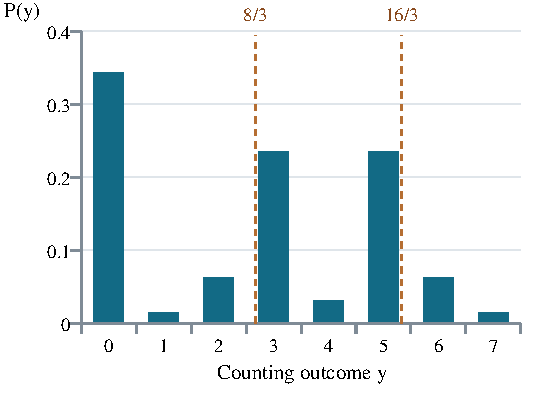
\includegraphics[width=\linewidth]{images/fourier-readout-q8-r3.pdf}
\end{minipage}
\end{center}
The peaks lie near \(0,8/3,16/3\). Yet
\[
(\rho_C')_{0,2}=\bra{\widetilde0}\rho_C\ket{\widetilde2}
=\frac{1-\ii}{64}\ne0.
\]
For this entry, summing \(\Gamma_c(0)\Gamma_c(2)^*\) gives \(-3\ii+3-2+2\ii=1-\ii\), and division by \(Q^2=64\) gives the result. Thus the inverse QFT leaves coherence while producing useful probabilities. The example illustrates structure; \(Q=8\) is too small for the usual general continued-fraction guarantee.

\phead{RECOVERING THE ORDER}{11. From a Fourier sample to factors}{Precision, repetition, and efficient gates complete the algorithm.}
Choose \(N^2\le Q=2^t<2N^2\). For a phase branch \(s/r\), let \(y\) be the closest grid point. Then
\[
\left|\frac yQ-\frac sr\right|\le\frac1{2Q}
<\frac1{2r^2},
\qquad r<N.
\]
The reduced fraction \(s/r\) therefore appears among the continued-fraction convergents of \(y/Q\). The geometric-sum law gives constant probability of a closest-grid-point outcome: for \(|\delta|\le1/(2Q)\),
\[
|D_Q(\delta)|^2
=\frac{\sin^2(\pi Q\delta)}{Q^2\sin^2(\pi\delta)}
\ge\frac4{\pi^2},
\]
using \(\sin u\ge2u/\pi\) on \([0,\pi/2]\) and \(|\sin v|\le|v|\). This is the usual conditional phase-estimation bound; one run still need not return a useful denominator.

If \(\gcd(s,r)=1\), the reduced denominator is \(r\); otherwise it is \(r/\gcd(s,r)\). Repeat and test candidates, or combine compatible denominators. The coprime fraction is \(\varphi(r)/r\). If \(k\) distinct primes divide \(r\), their ordered values satisfy \(p_i\ge i+1\), so
\[
\frac{\varphi(r)}r=\prod_{i=1}^k(1-1/p_i)\ge\frac1{k+1}\ge\frac1{1+\log_2r}.
\]
Thus polynomially many repetitions suffice. The outcome \(s=0\) is uninformative; arbitrary outputs need not be nearest-grid outcomes or useful order estimates.

Checking \(a^d\bmod N=1\) proves that \(d\) is a multiple of the true order; it does not by itself establish minimality. Test the candidate and the resulting gcd factors, and repeat when needed.

\lead{An example with standard precision}
Take \(N=21,a=2,Q=512\). Here
\[
r=6,\qquad(e_0,\ldots,e_5)=(1,2,4,8,16,11),
\]
\[
(M_0,\ldots,M_5)=(86,86,85,85,85,85).
\]
The peaks lie near \(y=0,85,171,256,341,427\). Suppose \(y=85\). Its continued fraction is
\[
\frac{85}{512}=[0;6,42,2],
\qquad
\frac16,\ \frac{42}{253},\ldots
\]
so \(1/6\) is a convergent. Verification gives \(2^6\bmod21=1\), and the even-order step yields
\[
\gcd(2^3-1,21)=7,\qquad\gcd(2^3+1,21)=3.
\]
Thus \(21=3\cdot7\).

\lead{Why the full procedure is polynomial}
With \(n=\lceil\log_2N\rceil\), we use \(t=O(n)\) control qubits, polynomial-size reversible modular arithmetic, an \(O(t^2)\)-gate exact QFT circuit, and polynomial-time continued fractions and gcd calculations. Repetition handles unsuccessful samples and choices of \(a\).
The QFT circuit follows the factorization
\[
F_Q\ket x=\bigotimes_{j=1}^{t}
\frac{\ket0+e^{2\pi\ii x/2^j}\ket1}{\sqrt2},
\]
with output qubits ordered from most to least significant. Hadamards and controlled phase rotations implement these factors, with swaps for the chosen wire order. Entanglement entropy alone is not a measure of computational advantage.

\phead{MEASUREMENT AND NOISE}{12. What is retained, ignored, or accidentally recorded?}{Orthogonal tags determine which local alternatives can interfere.}
\lead{Measuring the work register is optional}
A computational work measurement returning \(e_c\) has probability \(M_c/Q\) and leaves \(C\) in the pure comb \(\ket{C_c}\). Forgetting the outcome gives
\[
\sum_c\frac{M_c}{Q}\proj{C_c}=\rho_C,
\]
the same reduced state as never measuring \(W\). Measuring \(W\) in the \(U_a\) eigenbasis instead gives \(s\) with probability \(1/r\) and leaves \(\ket{\Phi_s}\). Forgetting \(s\) gives the same \(\rho_C\). These statements concern counting statistics; the joint states differ. Section 12a derives the separable unread state, unchanged comb coherence, and changed entropy and mutual information.

\lead{The final counting measurement}
Write
\[
\ket{\Psi_3}=\sum_y\ket y\ket{\chi_y},
\qquad
\ket{\chi_y}=\frac1Q\sum_c\Gamma_c(y)\ket{e_c}
=\frac1{\sqrt r}\sum_sD_s(y)\ket{u_s},
\quad \|\chi_y\|^2=P(y).
\]
Conditioned on a nonzero-probability outcome \(y\), the state becomes
\[
\ket y\otimes\frac{\ket{\chi_y}}{\sqrt{P(y)}}.
\]
Forgetting the outcome produces
\[
\sum_y\proj y\otimes\ket{\chi_y}\bra{\chi_y},
\quad
\rho_C^{\rm unread}=\sum_yP(y)\proj y.
\]
The counting measurement removes the computational off-diagonals when its outcome is forgotten. Its conditional joint state is product; its unread joint state is separable and mixed. The earlier pure-state entropy identities therefore no longer apply.

\lead{Scratch space: a general overlap rule}
For normalized scratch states \(\ket{g_x}\),
\[
\ket\Psi=\sum_x\alpha_x\ket x\ket{f(x)}\ket{g_x}
\quad\Longrightarrow\quad
(\rho_C)_{xx'}=\alpha_x\alpha_{x'}^*
\langle f(x')|f(x)\rangle\langle g_{x'}|g_x\rangle.
\]
The work factor retains coherence only within a period class. The scratch factor can suppress even that useful coherence. If scratch distinguishes every \(x\), then \(\langle g_{x'}|g_x\rangle=\delta_{xx'}\), giving a flat output for uniform \(\alpha_x\).
Uncomputation returns scratch to a common state. More generally it suffices not to distinguish alternatives within each residue class.

\lead{A simple noise model}
A depolarizing interpolation
\[
\rho_C(\eta)=\eta\rho_C+(1-\eta)\id_Q/Q,\qquad 0\le\eta\le1,
\]
gives \(P_\eta(y)=\eta P_{\rm ideal}(y)+(1-\eta)/Q\). For this particular uniform-diagonal input, partial computational dephasing gives the same interpolation. General noise is a channel \(\E(\rho)=\sum_jK_j\rho K_j^\dagger\), \(\sum_jK_j^\dagger K_j=\id\). After noise, local entropy generally includes environmental uncertainty and no longer equals the entanglement between \(C\) and \(W\).

\phead{PURE SUMS AND MIXED ENSEMBLES}{12a. Separability after a work measurement}{The same marginals can belong to an entangled pure state or a separable mixture.}
For a mixed joint state, separability means that at least one probabilistic product decomposition exists:
\[
\rho_{AB}=\sum_\alpha q_\alpha\,
\sigma_A^{(\alpha)}\otimes\tau_B^{(\alpha)},
\qquad q_\alpha\ge0,\quad\sum_\alpha q_\alpha=1.
\]
The local operators are normalized density matrices. Equivalently they may be pure projectors; their vectors need not be orthogonal. Such a state can be prepared using a shared random label and local preparations. Entangled means that no product-state ensemble reproduces the joint density matrix.

\lead{Why this reduces to Schmidt rank one for pure states}
If \(\rho_{AB}=\proj\Psi\), its support is one-dimensional. Positivity forces every pure vector in any ensemble for it to lie along the same ray \(\Psi\). A product ensemble is therefore possible exactly when \(\Psi\) itself factors:
\[
\text{pure and separable}\iff
\text{Schmidt rank }1\iff S(\rho_A)=S(\rho_B)=0.
\]
For mixed states, a spectral decomposition is only one possible ensemble. Entangled eigenvectors do not establish entanglement:
\[
\frac{\proj{00}+\proj{11}}2
=\frac{\proj{\Phi^+}+\proj{\Phi^-}}2,
\qquad
\ket{\Phi^\pm}=\frac{\ket{00}\pm\ket{11}}{\sqrt2}.
\]
The left side is explicitly separable. In the right side the Bell coherences cancel. A coherent sum of kets and a probabilistic sum of projectors have different meanings.

\lead{Apply the distinction to Shor's work measurement}
Write \(p_c=M_c/Q\) and \(h=H(p)=-\sum_cp_c\log_2p_c\). Before measurement,
\[
\ket{\Psi_2}=\sum_c\sqrt{p_c}\ket{C_c}\ket{e_c},
\qquad E=h,\quad S(CW)=0,\quad I(C:W)=2h.
\]
Measure \(W\) in the modular-value basis and forget the result. The resulting joint density matrix is
\[
\boxed{\rho^{\rm unread}_{CW}
=\sum_cp_c\,\proj{C_c}\otimes\proj{e_c}.}
\]
This is a separable mixture of orthogonal product states. Both marginals remain unchanged, but joint entropy is now \(h\), mutual information is \(h\), and \(C|W\) entanglement is zero. The local entropies still equal \(h\), demonstrating why they cease to measure inter-register entanglement once joint purity is lost.

Coherence between different Schmidt branches disappears, but coherence \emph{within} each periodic comb survives. Since \(\rho_C\) is unchanged, all subsequent counting-only statistics, including the inverse-QFT histogram, are identical. Entanglement need not persist between these two registers during readout.

This differs from completely dephasing \(C\) in its computational basis. That operation destroys within-comb coherence too, leaving \(\rho_C=\id_Q/Q\) and a uniform Fourier histogram. Likewise, a work eigenbasis measurement preserves \(\rho_C\), but generally changes \(\rho_W\) for \(r\nmid Q\); preservation of both marginals above uses the Schmidt/work-value basis.

\takeaway{For pure states, Schmidt rank and reduced entropy diagnose entanglement. For mixed states, local entropy or positive mutual information alone does not: separability concerns all possible product-state ensembles. Orthogonality is required for Schmidt spectral form, not for a separable mixed-state decomposition.}


\phead{REFERENCE: ALL DENSITY STAGES}{13. The entire evolution in parallel}{The ket and bra phases explain every density-matrix coefficient.}
Use \(\rho_j=\proj{\Psi_j}\), and write \(\ket{+_Q}=Q^{-1/2}\sum_x\ket x\). The work orbit basis \(E\) and modular eigenbasis \(U\) give the same operators:
\begingroup\eqsmall
\begin{align*}
\rho_0
&=\proj0\otimes\proj{e_0}
=\frac1r\sum_{s,t}\proj0\otimes\ket{u_s}\bra{u_t},\\
\rho_1
&=\frac1Q\sum_{x,x'}\ket x\bra{x'}\otimes\proj{e_0}\\
&=\frac1{Qr}\sum_{x,x',s,t}\ket x\bra{x'}\otimes\ket{u_s}\bra{u_t},\\
\rho_2
&=\frac1Q\sum_{x,x'}\ket x\bra{x'}\otimes
       \ket{e_{x\bmod r}}\bra{e_{x'\bmod r}}\\
&=\frac1{Qr}\sum_{x,x',s,t}\omega^{sx-tx'}
       \ket x\bra{x'}\otimes\ket{u_s}\bra{u_t}\\
&=\frac1r\sum_{s,t}\ket{\Phi_s}\bra{\Phi_t}\otimes\ket{u_s}\bra{u_t},\\
\rho_3
&=\frac1{Q^2}\sum_{y,y',c,d}\Gamma_c(y)\Gamma_d(y')^*
       \ket y\bra{y'}\otimes\ket{e_c}\bra{e_d}\\
&=\frac1r\sum_{y,y',s,t}D_s(y)D_t(y')^*
       \ket y\bra{y'}\otimes\ket{u_s}\bra{u_t}.
\end{align*}
\endgroup
The controlled phase acts on a matrix basis element by
\[
\ket x\bra{x'}\otimes\ket{u_s}\bra{u_t}
\longmapsto
\omega^{sx-tx'}\ket x\bra{x'}\otimes\ket{u_s}\bra{u_t}.
\]
The minus sign is complex conjugation of the bra amplitude. After \(\ell\) controlled multipliers replace \(sx-tx'\) by \(sp_\ell(x)-tp_\ell(x')\).

\lead{Reduce first, then apply the Born rule}
\[
(\rho_C')_{yy'}
=\frac1{Q^2}\sum_c\Gamma_c(y)\Gamma_c(y')^*
=\frac1r\sum_sD_s(y)D_s(y')^*,
\qquad P(y)=(\rho_C')_{yy}.
\]
All \(\rho_0,\ldots,\rho_3\) are pure joint states. The counting spectra at stages 0 and 1 are \((1,0,\ldots)\); at stages 2 and 3 they are \((M_0/Q,\ldots,M_{r-1}/Q,0,\ldots)\). The work state is unchanged by the local inverse QFT.

In work coordinates,
\[
[\rho_W]_E{}_{cd}=\frac{M_c}{Q}\delta_{cd},
\qquad
[\rho_W]_U{}_{st}=\frac1{Qr}\sum_x\omega^{(s-t)x}
=\frac1{Qr}\sum_cM_c\omega^{(s-t)c}.
\]
Thus \(U\) diagonalizes \(U_a\), not generally \(\rho_W\). Its measurement populations are always \(1/r\), while its coherences generally survive for \(r\nmid Q\). Uniform eigenphase outcomes are consistent with unequal Schmidt weights and entropy below \(\log_2r\).

\phead{APPENDIX: SIX PRODUCT BASES}{14. Complete bases and the initial stages}{A compact catalog, including the zero-eigenvalue directions that a support-only basis omits.}
The counting register has three useful coordinate systems:
\[
X=\{\ket x\},\qquad
F=\{\ket{\widetilde y}=F_Q\ket y\},\qquad
B=\{\ket{C_{c,\ell}}\},
\]
where the \emph{complete} comb basis is
\[
\ket{C_{c,\ell}}
=\frac1{\sqrt{M_c}}\sum_{m=0}^{M_c-1}
e^{2\pi\ii\ell m/M_c}\ket{c+mr},
\quad 0\le\ell<M_c.
\]
Write \(\alpha=(c,\ell)\), with \(\ket{C_c}=\ket{C_{c,0}}\).
Disjoint residue supports give orthogonality for different \(c\); for equal \(c\), the finite Fourier sum gives
\(\langle C_{c,\ell}|C_{c,\ell'}\rangle=\delta_{\ell\ell'}\).
Since \(\sum_cM_c=Q\), this is a full basis. Only \(\ell=0\) has nonzero pre-iQFT eigenvalues. The other \(Q-r\) directions are needed to express, for example, the initial \(\ket0\).

The work bases \(E=\{\ket{e_k}\}\) and \(U=\{\ket{u_s}\}\) each span the occupied \(r\)-dimensional orbit. Extend them outside the orbit for a full physical work-register basis; all amplitudes there are zero.

\lead{Stages 0 and 1: counting coordinates times work coordinates}
Both are products \(v_j\otimes\ket{e_0}\), where \(v_0=\ket0\), \(v_1=\ket{+_Q}\).
\begin{center}
\begin{tabular}{@{}lll@{}}
\toprule
Counting coordinates&\(\langle b_i|v_0\rangle\)&\(\langle b_i|v_1\rangle\)\\
\midrule
\(X,\ i=x\)&\(\delta_{x0}\)&\(1/\sqrt Q\)\\
\(B,\ i=(c,\ell)\)&\(\delta_{c0}/\sqrt{M_0}\)&\(\delta_{\ell0}\sqrt{M_c/Q}\)\\
\(F,\ i=y\)&\(1/\sqrt Q\)&\(\delta_{y0}\)\\
\bottomrule
\end{tabular}
\end{center}
Multiply each entry by \(\delta_{k0}\) for work coordinates \(E\), or by \(1/\sqrt r\) for coordinates \(U\). This specifies every initial and post-Hadamard ket in all six pairings, including all nullspace directions.

\lead{The overlaps needed for the remaining stages}
\[
\langle\widetilde y|C_c\rangle=\frac{\Gamma_c(y)}{\sqrt{QM_c}},
\qquad
D_s(y)=\frac1Q\sum_c\omega^{sc}\Gamma_c(y).
\]
Define \(G_{\alpha c}=\langle C_\alpha|F_Q^\dagger|C_c\rangle\). Explicitly,
\[
G_{(d,\ell),c}=
\frac1{\sqrt{QM_dM_c}}
\sum_{m=0}^{M_d-1}\sum_{n=0}^{M_c-1}
e^{-2\pi\ii\ell m/M_d}
e^{-2\pi\ii(d+mr)(c+nr)/Q}.
\]
It records the transformed comb in the original completed comb coordinates. It does not represent an additional physical gate.

\phead{APPENDIX: SIX PRODUCT BASES}{15. All post-ladder and post-iQFT amplitudes}{An amplitude table and one outer-product rule specify every ket and density matrix.}
For any chosen pairing write
\[
\ket{\Psi_j}=\sum_{i,k}A_j(i,k)\ket{b_i}\ket{w_k}.
\]
In the table, \(i=x\) in \(X\), \(i=(c,\ell)\) in \(B\), and \(i=y\) in \(F\).
Set \(p(y)=(-y)\bmod Q\).
\begingroup\tight
\begin{center}
\begin{tabularx}{\linewidth}{@{}lXX@{}}
\toprule
Pairing&After modular exponentiation: \(A_2\)&After physical inverse QFT: \(A_3\)\\
\midrule
\(X\otimes E\)&\(\displaystyle\frac{\delta_{k,x\bmod r}}{\sqrt Q}\)&
\(\displaystyle\frac{\Gamma_k(x)}Q\)\\[10pt]
\(X\otimes U\)&\(\displaystyle\frac{\omega^{sx}}{\sqrt{Qr}}\)&
\(\displaystyle\frac{D_s(x)}{\sqrt r}\)\\[10pt]
\(B\otimes E\)&\(\displaystyle\sqrt{\frac{M_c}Q}\delta_{\ell0}\delta_{kc}\)&
\(\displaystyle\sqrt{\frac{M_k}Q}\,G_{(c,\ell),k}\)\\[10pt]
\(B\otimes U\)&\(\displaystyle\sqrt{\frac{M_c}{Qr}}\delta_{\ell0}\omega^{sc}\)&
\(\displaystyle\sum_d\sqrt{\frac{M_d}{Qr}}G_{(c,\ell),d}\omega^{sd}\)\\[10pt]
\(F\otimes E\)&\(\displaystyle\frac{\Gamma_k(y)}Q\)&
\(\displaystyle\frac{\delta_{k,p(y)\bmod r}}{\sqrt Q}\)\\[10pt]
\(F\otimes U\)&\(\displaystyle\frac{D_s(y)}{\sqrt r}\)&
\(\displaystyle\frac{\omega^{sp(y)}}{\sqrt{Qr}}\)\\[5pt]
\bottomrule
\end{tabularx}
\end{center}
\endgroup
\lead{How to derive the table}
The \(X\otimes E\) row is the circuit itself. Expanding \(e_c\) into \(u_s\) gives \(X\otimes U\). Grouping \(x=c+mr\) gives \(B\otimes E\), and expanding its work tag gives \(B\otimes U\). Taking \(\bra{\widetilde y}\) overlaps gives the Fourier-coordinate rows. Applying the physical inverse QFT gives the right-hand column.

For the final two entries, Fourier coordinates contribute another mathematical \(F_Q^\dagger\):
\[
F_Q^{-2}\ket x=\ket{(-x)\bmod Q}.
\]
Thus post-gate Fourier coefficients are pre-gate computational coefficients with label \(p(y)\). There has been only one physical inverse QFT. For nondivisible \(Q\), reduce modulo \(Q\) \emph{before} modulo \(r\).

\lead{Generate every joint and reduced density matrix}
\[
\boxed{\begin{aligned}
[\rho_j]_{(i,k),(i',k')}&=A_j(i,k)A_j(i',k')^*,\\
[\rho_C^{(j)}]_{ii'}&=\sum_kA_j(i,k)A_j(i',k)^*,\\
[\rho_W^{(j)}]_{kk'}&=\sum_iA_j(i,k)A_j(i,k')^* .
\end{aligned}}
\]
For example, before iQFT,
\[
[\rho_C]_B{}_{(c,\ell),(d,m)}
=\frac{M_c}{Q}\delta_{cd}\delta_{\ell0}\delta_{m0},
\quad
[\rho_C]_F{}_{yy'}=\frac1{Q^2}\sum_c\Gamma_c(y)\Gamma_c(y')^*.
\]
The first is spectral and diagonal; the second supplies Fourier probabilities and is generally not diagonal. This catalog retains all six descriptions without repeating dozens of equivalent outer-product sums.

\phead{CONTEXT: THE ENTANGLEMENT NOTES}{16. Bell tests and Shor ask different questions}{The source notes' Bell argument, kept separate from the algorithmic mechanism.}
For a Bell pair \(\ket{\Phi^+}=(\ket{00}+\ket{11})/\sqrt2\), the global state is pure, each qubit is maximally mixed, \(E=1\) ebit, and \(I=2\) bits. A shared-coin mixture has the same marginals but \(S(AB)=1\), \(I=1\), and no entanglement. Thus neither local randomness nor nonzero mutual information by itself establishes entanglement.

\lead{A trusted entanglement witness is weaker than a Bell test}
For a product of qubit states, their Bloch components obey \(x_A^2+z_A^2\le1\) and \(x_B^2+z_B^2\le1\). Cauchy--Schwarz gives
\[
\langle X\otimes X\rangle+\langle Z\otimes Z\rangle
=x_Ax_B+z_Az_B\le1.
\]
Mixing preserves this bound for every separable state. The Bell pair gives \(2\), certifying entanglement when these are trusted Pauli measurements. An abstract classical response table can assign an answer to each question and agree in both bases. Two-basis agreement alone therefore does not exclude all local hidden-variable models.

\lead{Derive the CHSH constraint on local responses}
Let settings be \(x,y\in\{0,1\}\) and outcomes \(a,b\in\{\pm1\}\). A local shared-cause model, with setting independence, has
\[
p(a,b|x,y)=\int d\lambda\,p(\lambda)
p(a|x,\lambda)p(b|y,\lambda).
\]
It suffices to consider deterministic assignments, since stochastic local rules are mixtures of them. For each assignment,
\[
c=a_0(b_0+b_1)+a_1(b_0-b_1)=\pm2.
\]
One bracket is zero and the other is \(\pm2\). Averaging gives
\[
|\mathcal B|\le2,\qquad
\mathcal B=E_{00}+E_{01}+E_{10}-E_{11},\quad E_{xy}=\mathbb E[ab|x,y].
\]
For \(\Phi^+\), choose \(A_0=Z,A_1=X\), \(B_0=(Z+X)/\sqrt2\), and \(B_1=(Z-X)/\sqrt2\). Then \(E_{00}=E_{01}=E_{10}=1/\sqrt2\), \(E_{11}=-1/\sqrt2\), so \(\mathcal B=2\sqrt2\). These are qubit Bloch directions; photon polarizer angles use half these angular separations.

An experiment randomly chooses the settings at separated stations, records outcomes, and estimates all four averages, controlling detection bias and possible communication. Violation rules out the stated local model; it does not select an interpretation of when outcomes become real. Summing Bob's measurement effects gives the identity, so Alice's marginal is independent of Bob's setting: no faster-than-light signalling.

\lead{Why this distinction matters for the algorithm}
For \(\rho_p=p\proj{\Phi^+}+(1-p)\id_4/4\), entanglement begins at \(p>1/3\), but CHSH violation requires \(p>1/\sqrt2\). Shor's derivation instead uses its known pure joint state, Schmidt structure, and controlled interference. Its entanglement is certified by the model of the circuit; its useful output is a period estimate, rather than a Bell violation.

\phead{RECONSTRUCTION AND SOURCES}{17. What to derive from a blank page}{A short check that the representations connect rather than merely coexist.}
\begin{enumerate}[itemsep=1pt,topsep=2pt]
\item Derive every circuit stage, including intermediate controlled multipliers.
\item Prove the orbit eigenvectors, kickback, and the three descriptions of \(\Psi_2\).
\item Trace out work; relate the periodic-coherence matrix and Schmidt vectors to marginal spectra.
\item Count \(M_c\), normalize the combs, and distinguish rank, ebits, and mixed-state separability.
\item Derive both exact formulas for \(P(y)\); identify which amplitudes interfere.
\item Derive the ramp overlap, allowed Schmidt-basis rotations, and exact or broadened peaks.
\item Reconstruct and verify an order, then extract gcd factors.
\item Explain why work measurement can remove entanglement while preserving Fourier statistics, and why scratch records can destroy them.
\end{enumerate}

\lead{What was merged}
This explainer consolidates the two entanglement PDFs, eleven original pasted files (ten unique texts), the \(M_c\) derivation, the 69-page presentation, and the later Schmidt/separability chat. Sections 5a--5b and 12a integrate the new clarifications. Repeated arguments appear once; the basis catalog remains.

\begingroup\fontsize{9}{11.2}\selectfont
\begin{tabularx}{\linewidth}{@{}>{\raggedright\arraybackslash}p{0.55\linewidth}>{\raggedright\arraybackslash}X@{}}
\toprule
Supplied source or source group&Material retained\\
\midrule
\emph{shor\_pres\_v4\_1.pdf}, PDF pp. 25--49, 48--63; worked example pp. 42, 52&Cycle to spectrum, controlled kickback, free input, QPE linearity, orthogonal tags, matched filtering, four-branch example.\\
\emph{Entanglement: a short cheat sheet}; \emph{Entanglement, carefully defined} (Shor bridge)&States, partial traces, Bell/coin distinction, entropy, Shor, scratch and noise.\\
\emph{Understanding Shor's Algorithm}; \emph{Deriving Everything from Four Equations} (duplicate supplied twice)&Unified derivations and equivalence of periodic, phase, Schmidt, and Fourier descriptions.\\
\emph{One-night mastery plan}; conversation summary&Motivation, diagnostic questions, reconstruction exercises.\\
Comb-eigenbasis clarification; \emph{Why the inverse QFT reveals Shor's period without necessarily diagonalizing}&Degeneracy, measurement labels, active/passive distinction, nondivisible counterexample.\\
\emph{Through State Vectors and Density Matrices}; four-pairing recommendation&Parallel ket/matrix explanations and selection of the main conceptual views.\\
\emph{All Six Product Bases}; \emph{Complete State Evolution in Parallel}&Complete basis catalog, all physical stages, joint/reduced matrix formulas.\\
Current \(M_c\) and \(\log_2r\) addition&Exact class counts, unequal Schmidt weights, rank versus ebits, \(I=2E\).\\
Later Schmidt/separability chat&Equivalent entanglement descriptions; orthogonality, marginal spectra, degenerate rotations, ramp overlaps, and separable unread work measurements.\\
\bottomrule
\end{tabularx}
\endgroup

\lead{Primary references for the underlying results}
\begingroup\fontsize{9}{11.2}\selectfont
P. W. Shor, \emph{Polynomial-Time Algorithms for Prime Factorization and Discrete Logarithms on a Quantum Computer}, \href{https://arxiv.org/abs/quant-ph/9508027}{arXiv:quant-ph/9508027}. The circuit and number-theoretic recovery derive from this order-finding method.

J. Preskill, \emph{Quantum Shannon Theory}, \href{https://arxiv.org/abs/1604.07450}{arXiv:1604.07450}. For entropy, relative entropy, mutual information, and their operational meanings.

C. H. Bennett et al., \emph{Concentrating Partial Entanglement by Local Operations}, \href{https://arxiv.org/abs/quant-ph/9511030}{arXiv:quant-ph/9511030}. For the asymptotic Bell-pair meaning of pure-state entanglement entropy.

J. F. Clauser et al., \emph{Proposed Experiment to Test Local Hidden-Variable Theories}, \href{https://doi.org/10.1103/PhysRevLett.23.880}{Physical Review Letters 23, 880 (1969)}. For the CHSH test.
\endgroup
\label{docend}
\end{document}
